\chapter{Cetacean Detection Using Deep Learning}\label{ch:cetDet}

When building any large-scale project, it is important to break the task down into various subcomponents. This chapter examines one such subcomponent utilised in the development of an automatic photo-id system, the cetacean detector. This component takes images captured during photo-id surveys and locates regions of interest (RoIs) -- defined as areas in which a dorsal fin breaches the waterline. This chapter will discuss the requirements a detector must meet, as well as its training and hyperparameter optimisation. 

\section{Requirements of a Cetacean Detector}\label{ch:cetDet,sec:requirements}

Before a system for automatic cetacean detection can be developed, it is important to first define the problem and understand the requirements of the system. The overall aim of the detector is to be able to take large-scale images as input, fed in one at a time, and process them in order to locate RoIs. This detector will only be required to identify one object class, dolphins. These detected regions can then be passed further down the system pipeline for photo-identification. 

 As such, this detector can be considered a coarse-grained task, and at first glance may seem somewhat trivial. However due to both the nature of the environment in which the RoIs must be detected, and the technical requirements the system must perform under, this is actually a complex problem. 
 
 \subsection{Environmental Requirements}\label{ch:cetDet,sec:requirements,sub:environmental}
 
 Firstly the area in which this system is to be deployed, open water, is susceptible to adverse weather conditions such as high winds. This in turn leads to sub-optimal conditions for detection which the system must be capable of handling, most notably high amounts of sea swell. Further to this, cetaceans are communal and travel in pods. An example of this behaviour can be seen in Figure \ref{fig:pod-eg}. Thus, the system must be capable of differentiating between overlapping individuals. Even if not all of the overlapping individuals are suitable for identification downstream, the system must still be able to separate them into individual detections to prevent misclassification.
 
 \begin{figure}
 	\begin{center}
 		\includegraphics[scale=0.06]{Chapter4/figs/dolphins-in-pod-example.JPG}
 	\end{center}
 	\caption{Some cetaceans, such as bottlenose dolphins, travel in pods. The developed detection system must be capable of splitting this pod into individual animals to be passed to the identifier.
 	}
 	\label{fig:pod-eg}
 \end{figure}

 Next, the detector must be capable of differentiating between dolphin fins and waves. Again this might sound trivial, but thousands of years of evolution have resulted in fins and waves looking extremely similar to the untrained (artificial) eye. Especially from a distance and in choppy waters, fins and waves often have extremely similar shape and structure. Furthermore, the animal's bodies are also similarly coloured to their surroundings. These adaptations allow the animals to be better protected and camouflaged in their environment, but can cause issues with detection systems. This becomes apparent when thinking about how CNNs \textit{see}. As described in Chapter \ref{ch:Background,sec:DLforCV}, CNNs see input images as a matrix of pixel values. When training an object detection system the CNN is told which parts of this matrix are related to a class -- any without a class label are considered background. If fins and areas of background contain similar pixel values, and these pixel values are clustered in similar ways, this can result in issues when training a model to detect instances of a class without misclassifying the background. 
 
 Another important requirement is for the detector to be able to handle objects of varying size, shape, direction, and angle of approach. When working in an open water environment with live animals, there is no guarantee how the animal will approach the camera, and thus the detector must be generalisable enough to handle this. 
 
 Furthermore, how the animals breach the water is also extremely variable. Breachings may occur in any direction relative to the boat and the animal could itself be travelling in a different cardinality. The ideal scenario would be for a breaching to occur either directly East or West of the boat (off the port or starboard side respectively) with the animal travelling perpendicular as this provides the best chance for researchers, who often position themselves to capture from these sides to minimise photographing parts of the vessel, to capture markings -- however this rarely occurs. For example, a breaching may occur off the port-side of the bow (approx North West relative to the boat), but the animal may be travelling in a South-Easterly direction. These approaches greatly change the look of the fin, although they may still contain identifiable markings. The detector should be able to detect these fins and pass them along for identification. An example of this can be seen in Figure \ref{fig:angle-eg}, which also shows how distance from the vessel can change the camera's view of the dorsal. 
 
   \begin{figure}
 	\begin{center}
 		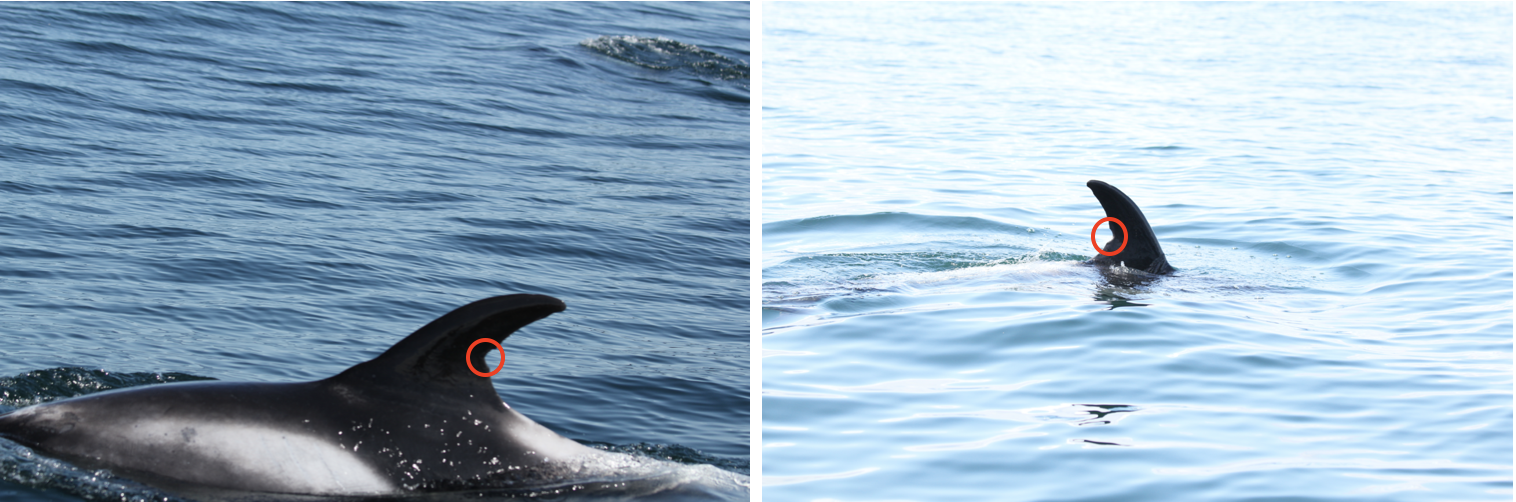
\includegraphics[scale=0.6]{Chapter4/figs/angle-size-example.png}
 	\end{center}
 	\caption[Two images of the same individual taken from different angles of approach, directions of travel, and distances from the vessel.]{Two images of the same individual taken from different angles of approach, directions of travel, and distances from the vessel. Note how this changes the make-up of the dorsal fin but keeps the identifying notch, highlighted, visible. 
 	}
 	\label{fig:angle-eg}
 \end{figure}
 
 As mentioned previously, weather conditions can also greatly affect how a dorsal fin is captured by a camera. However in photo-id surveys there are only two conditions that need to be worried about; swell and lighting. This is due to most research groups limiting travel in rough seas for safety reasons. Within Newcastle University's Marine MEGAfauna Lab for example, this limit is a sea state $<4$ on the Beaufort Sea State scale \cite{world_meteorologicial_society_beaufort_1970}. As such, a mild amount of swell and splash can be expected which the detector should be capable of handling. Lighting conditions are not considered in the Beaufort scale, but for operational reasons the vast majority of photo-id surveys take place during daylight hours. This can lead to large amounts of glare in images, especially on clear days. The detector should be invariant to these conditions. 
 
 \subsection{Technical Requirements}\label{ch:cetDet,sec:requirements,sub:technical}
 
On top of being able to handle a variety of environmental factors, there are also some technical requirements that the detector must meet. As outlined in Chapter \ref{ch:Background}, this thesis makes use of deep computer vision approaches. When using these types of tools, there is often a trade off that must be made between speed and accuracy. In most cases, these are inversely proportional to each other; the faster a system is required to perform, the lower an accuracy you must be willing to tolerate -- Huang \textit{et al.} discuss this in greater detail \cite{huang_speedaccuracy_2017}.
 
 Because this trade off must be made, it is important to decide where a deep learning model will be utilised before it is deployed. As photo-id surveys are performed on small vessels such as Rigid Inflatable Boats (RIBs), space is severely limited on board. As such, it is not appropriate to add additional hardware to the vessel to perform this analysis during the survey. Furthermore, the current methodology of cetacean researchers is to perform identification once back on land, even when utilising photo-id aids. As the system proposed in this thesis is intended to fit into existing procedures rather than replace them, it is appropriate for the system to be land based rather than on the vessel. Thinking about the current procedure further, this thesis' proposed system could be, for example, left running overnight performing identifications whilst the researchers are asleep or during the day whilst they are on another survey. As such, there is no need for the system to operate in real-time to fit in with the current workflow of cetacean researchers provided the system completes its task within a reasonable time frame. Further to this, as the output of the detection model will be passed to an identification model, it is imperative that as much noise, defined as any non-animal related nuisance such as splash, waves, and other vessels, is removed as possible during the detection. In order to do this, the accuracy of the detection must be as high as possible, furthering the case for an accurate system over a fast one.
 
 This idea of reducing as much noise as possible can be used to further narrow down the requirements of the detection system. As discussed in Section \ref{ch:Background,sec:DLforCV}, the output of detection systems can be provided in different formats. In bounding box detection systems the detected objects are described by a set of at least two pixel coordinates denoting the top-left and bottom-right extremes of the object. These detections are often more cost-effective, both from a labelling perspective requiring less person-hours to complete, and to perform computationally. Bounding box-based detections are limited in their ability to remove background noise however, with only the background outside of the box removed.
 
 If pixel-wise mappings are utilised, then each pixel is given a classification. This allows the system to be more discrete with its detection, allowing for the removal of as much background as possible. Both semantic (one mask for all objects of the same class) and instance (one mask for each object of a class) segmentation methods allow the detector to utilise pixel-wise mappings to remove background noise. Pixel-wise labelling is far more labour intensive and costly to produce compared to bounding box labelling. Utilising the requirements as defined in Section \ref{ch:cetDet,sec:requirements,sub:environmental}, specifically that the detector must be capable of reducing an overlapping pod to its individual component animals, the use of pixel-wise mappings at an instance level would be preferable over semantic or bounding box level detections. This requirement reveals a further trade-off the system must make. The amount of noise removed by the detector is proportional to the cost and labour needed to create data to train the system. This is discussed in more detail in Section \ref{ch:cetDet,sec:deciding,sub:boundingBoxInvestigation}.
 
 Furthermore, any system performing cetacean detection from photo-id survey data must be capable of working with large scale images. In most image based tasks where deep learning is utilised, images fed to the network are downscaled to allow for faster training and a reduction in overall network size. Downscaling images reduces the number of pixels in the image, which by definition reduces the amount of information present as pixel values need to be pooled (one pixel needs to now display what multiple would have previously). For most detection tasks this would not be an issue, and indeed if this thesis' goal was solely cetacean detection there would be no issues with downscaling. This detector is not stand-alone however but rather the first stage of a pipeline of networks with the end goal of photo-identification. The identification task relies on potentially minute details in the fin such as notches; any downscaling of the image at the detection stage runs the risk of removing potentially identifiable information in the fin. As such, the image must only be reduced in size once it is certain that no identifying information will be lost. As this cannot be guaranteed at the stage of detection, the detector must be capable of operating on images without resizing.
 
\section{Deciding on Approach}\label{ch:cetDet,sec:deciding}

Based on the requirements outlined in Section \ref{ch:cetDet,sec:requirements}, it is possible to begin deciding on how the cetacean detector is to be developed. One of the most important factors in the overall approach taken in the detector's development, and ultimately the overall automatic photo-id system, would be the use of either bounding boxes or pixel-wise mappings. As mentioned previously, the use of pixel-wise mappings would allow for a greater removal of background noise, but is extremely costly and labour intensive to produce. In contrast, bounding box labels are easier and cheaper to produce but will lead to less background noise removal. 

\subsection{An Investigation into Bounding Boxes}\label{ch:cetDet,sec:deciding,sub:boundingBoxInvestigation}

Due to their relative cheapness and ease to produce, the use of bounding boxes would be extremely beneficial. However, if the use of bounding boxes at this stage would hinder the accuracy of individual identification downstream, then this would outweigh the cost of pixel-wise mappings. 

As such, an investigation was undertaken to decide whether bounding boxes would be a viable option or if their use would hinder downstream identification. To begin, a small subset of the Zanzibar dataset, discussed in more detail in Section \ref{ch:datasetCreation,sec:zanzibar}, was manually cropped to simulate the output of a bounding box detector, an example of which can be seen in Figure \ref{fig:manual-crop-example}. This manually cropped data included some background but ensured the RoI, the dorsal fin, was centred and prominent representing an optimal output from a bounding box detector. 

\begin{figure}
	\begin{center}
		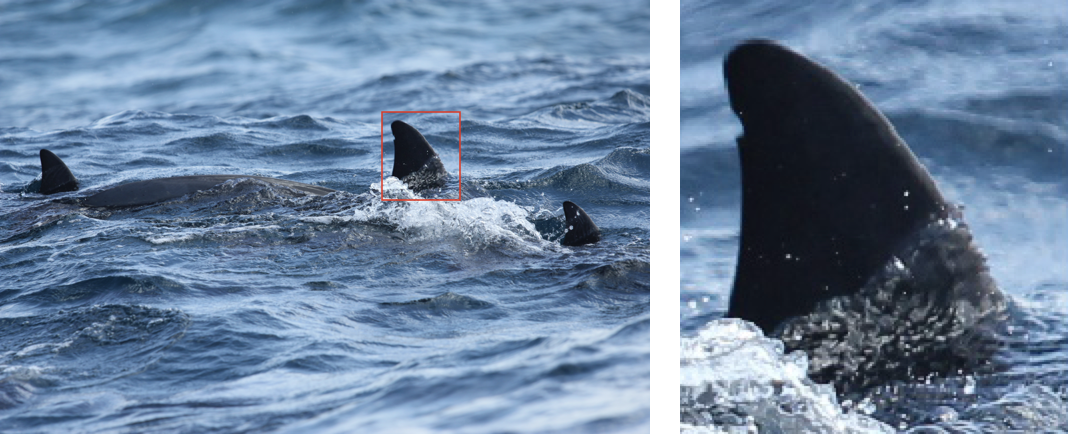
\includegraphics[scale=0.6]{Chapter4/figs/manual-crop-example-updated.png}
	\end{center}
	\caption[Left: an example input image. Right: the corrsponding manual crop utilised in bounding box suitability testing.]{Left: an example input image. Right: the corrsponding manual crop utilised in bounding box suitability testing. The RoI used to produce the manual crop is highlighted red in the input image.}
	\label{fig:manual-crop-example}
\end{figure}

\subsubsection{Feature Extraction with SURF}\label{ch:cetDet,sec:deciding,sub:boundingBoxInvestigation,subsub:SURF}

To begin, processing of the cropped images focussed on the use of feature extractors such as SURF \cite{bay_speeded-up_2008}. Like its predecessor SIFT \cite{lowe_object_1999}, SURF is invariant to scale, a major advantage for use with cetacean survey data where the RoI's size may change depending on when the image of the dorsal fin breaching the water is captured. If SURF was capable of producing feature descriptors of the dorsal fins with only partial background removal, this would show potential for individual identification where some background is present, possibly through the use of the feature descriptors.

First SURF was performed over the entire cropped image. This proved unfruitful however, picking out relatively few features in areas of the image which contained the animal's dorsal fin and instead focussing on the feature heavy areas present in the sea -- an example of this can be seen in Figure \ref{fig:manual-crop-surf-example}. This result indicated that further refinement was required, potentially reducing the area SURF was allowed to explore.

\begin{figure}
	\begin{center}
		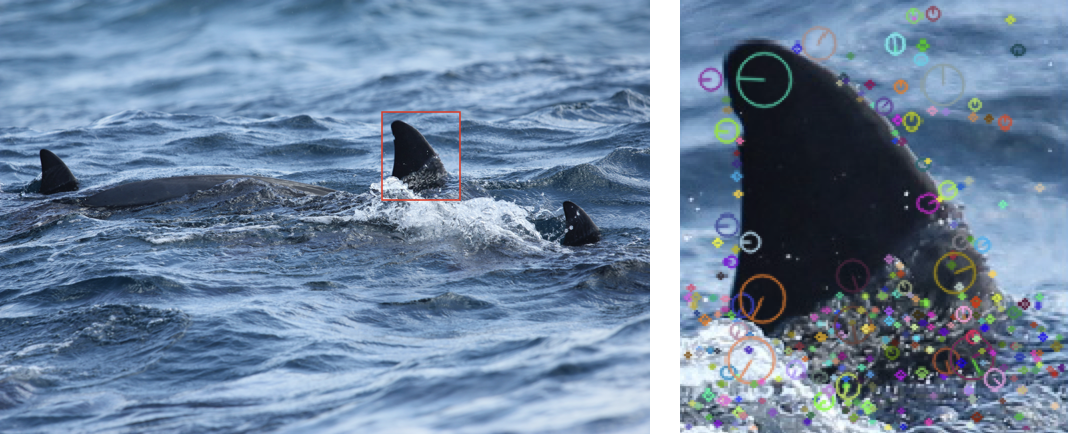
\includegraphics[scale=0.6]{Chapter4/figs/manual-crop-surf-updated.png}
	\end{center}
	\caption[Left: an example input image. Right: the corresponding manual crop with the result of SURF feature extraction overlaid.]{Left: an example input image. Right: the corresponding manual crop with the result of SURF feature extraction overlaid. The majority of features extracted are from the surrounding background water. The RoI used to produce the manual crop is highlighted red in the input image.}
	\label{fig:manual-crop-surf-example}
\end{figure}

Reduction of the search space available to SURF was achieved through the use of colour thresholding. As such, SURF would only be performed in areas of the image where pixel values fell within some defined range. Here, a mask was created programmatically for each image based on bounded RGB colour values found in the dorsal fins, giving an upper threshold of (14, 16, 26) and a lower threshold of (54, 51, 66) -- see Section \ref{ch:Background,sec:DLforCV} for a description of the RGB colour space. An example result of SURF after colour thresholding can be see in Figure \ref{fig:manual-crop-surf-colour-thresholding-example}, with coloured circles surrounding extracted features. As can be seen, colour thresholding helps in removing a large amount of background water from the computation. Issues arise however where areas of water are also within the threshold's bounds. Because of this, colour thresholding before SURF only reduces the amount of features extracted from the water, it does not remove them, which may result in misidentification downstream.

Further to this, it can be seen that SURF is incapable of extracting relevant prominent markings from the species in the image, Indo-Pacific bottlenose dolphins (\textit{Tursiops aduncus}). For example, in Figure \ref{fig:manual-crop-example}, a notch is clearly present on the dorsal fin which is a good marker for individual identification. However, when performing SURF on this dorsal as seen in Figure \ref{fig:manual-crop-surf-colour-thresholding-example}, note how this notch has not been detected by SURF, which has instead detected an area above the notch which contains no identifiable information. 

\begin{figure}
	\begin{center}
		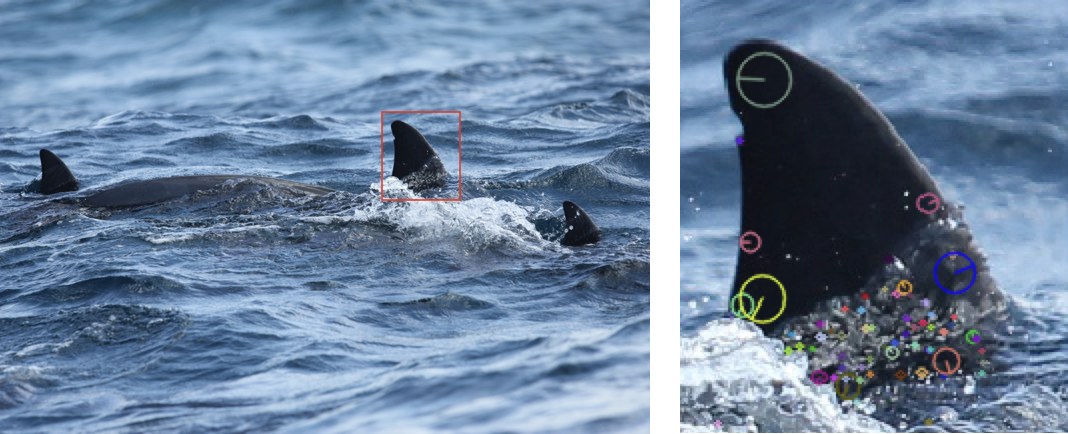
\includegraphics[scale=0.6]{Chapter4/figs/manual-crop-surf-colour-thresholding-axis.png}
	\end{center}
	\caption[Left: an example input image. Right: the corresponding manual crop with the result of SURF feature extraction when thresholded based on RGB colour values overlaid.]{Left: an example input image. Right: the corresponding manual crop with the result of SURF feature extraction when thresholded based on RGB colour values overlaid. A large number of features have been extracted from splash surrounding the dorsal fin, alongside few identifying features. The RoI used to produce the manual crop is highlighted red in the input image.
	}
	\label{fig:manual-crop-surf-colour-thresholding-example}
\end{figure}

Feature extraction methods such as SURF are also incapable of extracting other identifiable markers such as fin shape. As such, the use of feature extractors was deemed improper for this use case. It is important to note here that the use of feature extractors may be appropriate for cetacean species other than this project's data subjects of bottlenose and white-beaked dolphins. For example, the use of both SURF and SIFT has been shown to be appropriate to aid in identification of individual Risso's dolphins \cite{reno_sift-based_2019, maglietta_dolfin_2018}.

\subsubsection{Background Removal with GrabCut}\label{ch:cetDet,sec:deciding,sub:boundingBoxInvestigation,subsub:GrabCut}

Testing the suitability of SURF as described in Section \ref{ch:cetDet,sec:deciding,sub:boundingBoxInvestigation,subsub:SURF} highlighted the need for complete background removal before identification. In order for bounding boxes to be a viable option in this scenario, a robust background removal process would need to be created. Further, the process would need to be capable of operating under unseen conditions in an unsupervised manner without pixel labelled data to train on. If the background removal process required training data to operate, this would increase the overall cost and labour required to use bounding boxes, and as such reduces the suitability of them compared to utilising pixel-wise mappings from the beginning.

GrabCut, an algorithm proposed by Microsoft Research \cite{rother_grabcut_2004}, allows for the segmentation of foreground objects from the background with minimal or no human interaction. As GrabCut would be utilised in a fully automated setting, the algorithm would be required to perform background removal with no human interaction. Testing of the suitability for GrabCut was performed using the same cropped images as those used for SURF testing. Again, issues arose when performing GrabCut on the cropped image data. The algorithm struggled to understand which parts of the image were background and foreground, resulting in imperfect segmentations. This was especially an issue where the dorsal fin was present in rough water, where splash would be in front of the dorsal fin when captured by the camera. The use of GrabCut on Figure \ref{fig:manual-crop-example} can be seen in Figure \ref{fig:grabcut-example}.

\begin{figure}
	\begin{center}
		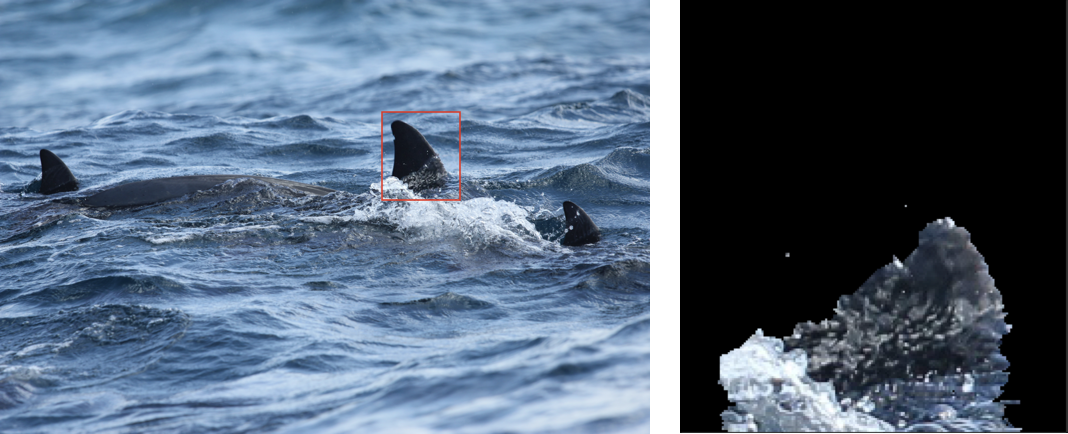
\includegraphics[scale=0.6]{Chapter4/figs/grabcut-example-updated.png}
	\end{center}
	\caption[Left: an example input image. Right: the corresponding manual crop with the result of GrabCut background removal overlaid.]{Left: an example input image. Right: the corresponding manual crop with the result of GrabCut background removal overlaid. A large portion of the dorsal fin has been discarded, having been deemed a background object due to the foreground splash. The RoI used to produce the manual crop is highlighted red in the input image.
	}
	\label{fig:grabcut-example}
\end{figure}

As can be seen, the use of GrabCut as a background removal tool does not perform as expected on data the detector is required to operate on. Because of this, as well as the unsuitability of feature extraction as seen in Section \ref{ch:cetDet,sec:deciding,sub:boundingBoxInvestigation,subsub:SURF}, the use of bounding boxes in the cetacean detector stage was deemed improper. As such, the focus of testing moved to the use of pixel-wise mappings and instance segmentation.  

\subsection{Instance Segmentation Architectures}\label{ch:cetDet,sec:deciding,sub:instanceSegArchitectures}

One of the major decisions to be made is which model architecture should be utilised in order to provide the required pixel-level detections. As this thesis is devoted to improving existing procedures and introducing deep learning to a novel application domain, it is far more advantageous to utilise existing model architectures rather than develop a custom one -- it would not be appropriate to develop a new approach from scratch should an existing one achieve the desired outcome. The development of a custom architecture for this stage of the project would also be extremely time consuming, taking away from more novel parts of the project (notably the identification of the individual animals). Further, as this project is introducing deep learning methods to an application domain where it is not commonplace, the project needs to be able to convince researchers in the space that the system is reliable; this is more easily achieved using a pre-existing architecture where use cases already exist in the literature. 

To this end there are two main model architectures that can be considered for this task; U-Net \cite{ronneberger_u-net_2015} and Mask R-CNN \cite{he_mask_2017}. Both of these architectures work in different ways. Vuola \textit{et al.} provide a more detailed comparison between the two models \cite{vuola_mask-rcnn_2019}, however the main focus for this thesis is their resultant output mask structure. 

U-Net is based on an encoder-decoder architecture. This allows for fast and simple segmentation when working with images where only one output is required. For example taking U-Net's original use case of biomedical imaging, the model is able segment a group of cells efficiently into individual components through boundary estimation to locate the outer edges of the cells. This allows them to be segmented from each other. However this results in an output of the same dimensions as the input, that is, all segmentations are provided in a single binary mask. 

In contrast, Mask R-CNN utilises a multi-stage architecture (described in more detail in Section \ref{ch:Background,sec:instanceSegmentation,sub:Mask R-CNN}) allowing the model to place each detection on its own binary output mask. This is extremely important for the outlined use case. As the detector will be used as part of a larger system for automatic photo-id, any detections made will need to be passed to the identifier as a stand-alone image. If U-Net was utilised for the detection stage, whilst initially being more efficient than Mask R-CNN, further processing of the binary output mask would still be required to split this into its individual components. In contrast, if Mask R-CNN was utilised then the processing required between the detection and identification stage would be far simpler. Again, this allows for more time to be spent working on the novel aspects of this thesis whilst keeping the pipeline as simple as possible. These outlined reasons were a major factor in deciding to focus on Mask R-CNN for this stage in the pipeline.

\section{Initial Testing of Mask R-CNN}\label{ch:cetDet,sec:initialTesting}

The following sections detail the creation of the Mask R-CNN based cetacean detector. Figure \ref{fig:pipeline-detector} highlights where in the system pipeline this model will be placed.

\begin{figure}[!h]
	\begin{center}
		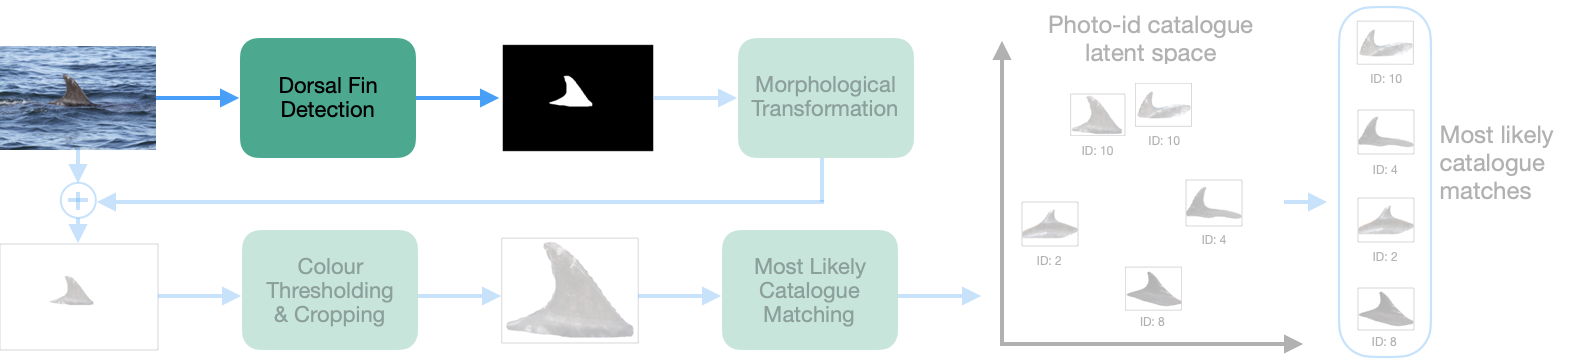
\includegraphics[width=\linewidth]{Chapter4/figs/pipeline-detector.png}
	\end{center}
	\caption[The high level pipeline overview, shown in Figure \ref{fig:pipeline}, with the Mask R-CNN component highlighted.]{The high level pipeline overview, shown in Figure \ref{fig:pipeline}, with the Mask R-CNN component highlighted. It is this part of the pipeline that will be discussed in the following Sections.}
	\label{fig:pipeline-detector}
\end{figure}

Rather than developing a custom Mask R-CNN implementation for this project, Matterport's repository \cite{waleed_mask_2017} was adapted. To determine the suitability of a Mask R-CNN based model for the task of a cetacean detector, the Zanzibar dataset was divided randomly using an 80-20 split, where 80\% of the images are designated for training the Mask R-CNN model, known as the training set, and the remaining 20\% were held back for model evaluation, known as the test set. By evaluating on previously unseen data this affords researchers the ability to understand the generalisability of the trained model, mitigating overfitting.

\subsection{Transfer Learning}\label{ch:cetDet,sec:initialTesting,sub:transferLearning}

Whilst the Zanzibar dataset provides experimental data similar to that which the Mask R-CNN model will be required to process, the amount of data is extremely small. Deep learning models often require thousands of images when training to produce generalisable and accurate models. As such, this dataset alone would not be enough to train the cetacean detector. One way to approach this issue would be to locate more photo-id data. However, little extra data were readily available from the Marine MEGAfauna Lab, and data from other labs was deemed too costly to obtain. Cetacean catalogues are closely guarded by research labs due to the large amount of effort required to obtain them. Second, any further data collected would also need to be labelled and incorporated into the now existing dataset, which again would require significant time and effort. These issues rendered the prospect of expanding the Zanzibar dataset unachievable in the time required. 

Another approach available is the concept of transfer learning. This is a technique whereby models trained to perform one task are repurposed to aid in a second, usually more specialised task. These initial models have typically been trained on large generalised datasets such as ImageNet \cite{deng_imagenet:_2009} or Microsoft's Common Objects in Context, more commonly known as MSCOCO \cite{lin_microsoft_2014}. These datasets often contain hundreds of thousands of images covering a large number of classes, which make them perfect for the task of transfer learning. 

By first training a model on these large datasets, the model is able to learn the basics of image understanding, for example the concept of basic shapes and colour, allowing for the development of a generic visual understanding model. Through this, the model is effectively given a head start in its learning process as there is no need to utilise the small amount of data available in the Zanzibar dataset for low level learning; it can instead be saved for allowing the model to understand and generalise to the domain-specific task, such as cetacean detection. For a more in-depth analysis of transfer learning, see Pan \textit{et al.} \cite{pan_survey_2010}.

Training a neural network, or model, is extremely computationally and time expensive due to the large dataset sizes used. As such, many models suitable for transfer learning can be obtained in a pre-trained state. These pre-trained models are hosted by model zoos, which provide frozen model weight files in a format which allows for transfer learning to take place through a process known as fine-tuning. Here, a model from the zoo is downloaded and \textit{N}-number of deeper layers are unfrozen. Next, additional layers are added to the model which perform the domain-specific task. The unfrozen and additional layers are then trained on the domain-specific task, allowing for the fine-tuning of the higher-level feature extraction. 

\subsection{Utilising Transfer Learning to Train the Mask R-CNN}\label{ch:cetDet,sec:initialTesting,sub:transferLearningforTheDetector}

The use of transfer learning can be easily adapted for the training of the cetacean detector for use with the Zanzibar dataset. First, a backbone model architecture is chosen. For the cetacean detector, it was decided that a ResNet50 \cite{he_deep_2015} backbone would be utilised. This was chosen over ResNet101 as during initial experimentation, no significant improvement in accuracy was achieved using the deeper 101 layer model although a significant increase in training time was observed.

Next, the pre-trained model weights are passed to the chosen architecture from the model zoo. These weights denote the strength of the connections between the model's layers. In the case of a model being trained from scratch without transfer learning, the weights of each layer are randomly initialised and then manipulated through backpropagation to achieve a desired model output. In transfer learning however, the model's starting weights are not initialised randomly. Instead, the weights of the trained network hosted on the model zoo are used as a starting point. This replicates the final state of the model trained on the larger dataset. 

As previously mentioned, there are multiple different models available in the zoo, all trained on a large variety of benchmark datasets. This work makes use of MSCOCO \cite{lin_microsoft_2014} for model pre-training. This is due to the fact that MSCOCO is primarily an instance segmentation dataset, and thus one of the most appropriate to use for transfer learning to another instance segmentation task. The use of MSCOCO for pre-training on R-CNN models has in recent years been well documented in literature for a variety of tasks \cite{yu_fruit_2019, couteaux_automatic_2019, fujita_fine-tuned_2020} including in land-based photo-id systems, with Kulits \textit{et al}. utilising MSCOCO as a transfer learning dataset when training a modified Faster-RCNN system for African elephant re-identification \cite{kulits_elephantbook_2021}. As Mask R-CNN builds on Faster-RCNN, it was deemed reasonable to assume MSCOCO would also work well for pretraining a Mask R-CNN based system.

Whilst it may at first seem to make sense to pre-train on large scale natural datasets such as iNaturalist \cite{van_horn_inaturalist_2018}, it is important to note that datasets such as these often contain example images of classes in an `iconic' view. If class overlap exists between the pre-training and target datasets, where objects in the latter are shown in a variety of views, this may bias the learning process \cite{pantazis_focus_2021}. By utilising a pre-training dataset where no class overlap with the target exists, the potential for object view bias is negated. 

When utilising an MSCOCO pre-trained architecture for a Mask R-CNN based task, it is important to note that certain layers must be excluded when loading in the pre-trained weights as these are only utilised in Mask R-CNN models, such as those which deal with the per-pixel masks. This is because these layers require the same number of neurons as dataset classes, similar to a fully connected layer. If the MSCOCO weights were utilised at these final layers for the task at hand there would be a mismatch between the number of classes in MSCOCO, 80, and in the Zanzibar dataset, 1 (plus background).

Once the backbone architecture has been loaded with pre-trained weights, the total number of layers to fine-tune must be decided. This can be considered similar to a hyperparameter, as it must be chosen at run time by the user. Whilst any number of the layers can be chosen for fine-tuning, only the model heads are selected. These are layers required for the Region Proposal Network, the pixel classification, and masking layers of the model. Whether model weights are randomly initialised or loaded from a pre-trained model is determined during hyperparameter tuning.

\subsection{Data Augmentation}\label{ch:cetDet,sec:initialTesting,sub:dataaugmentation}

As well as transfer learning, the use of data augmentation was also explored to help mitigate the issue of dataset size. This technique allows for datasets to be artificially expanded by performing random perturbations to each data point which are then automatically class labelled the same as the original input. Figure \ref{fig:data-aug-examples} shows examples of data augmentations found in the literature.

\begin{figure}[h]
	\begin{center}
		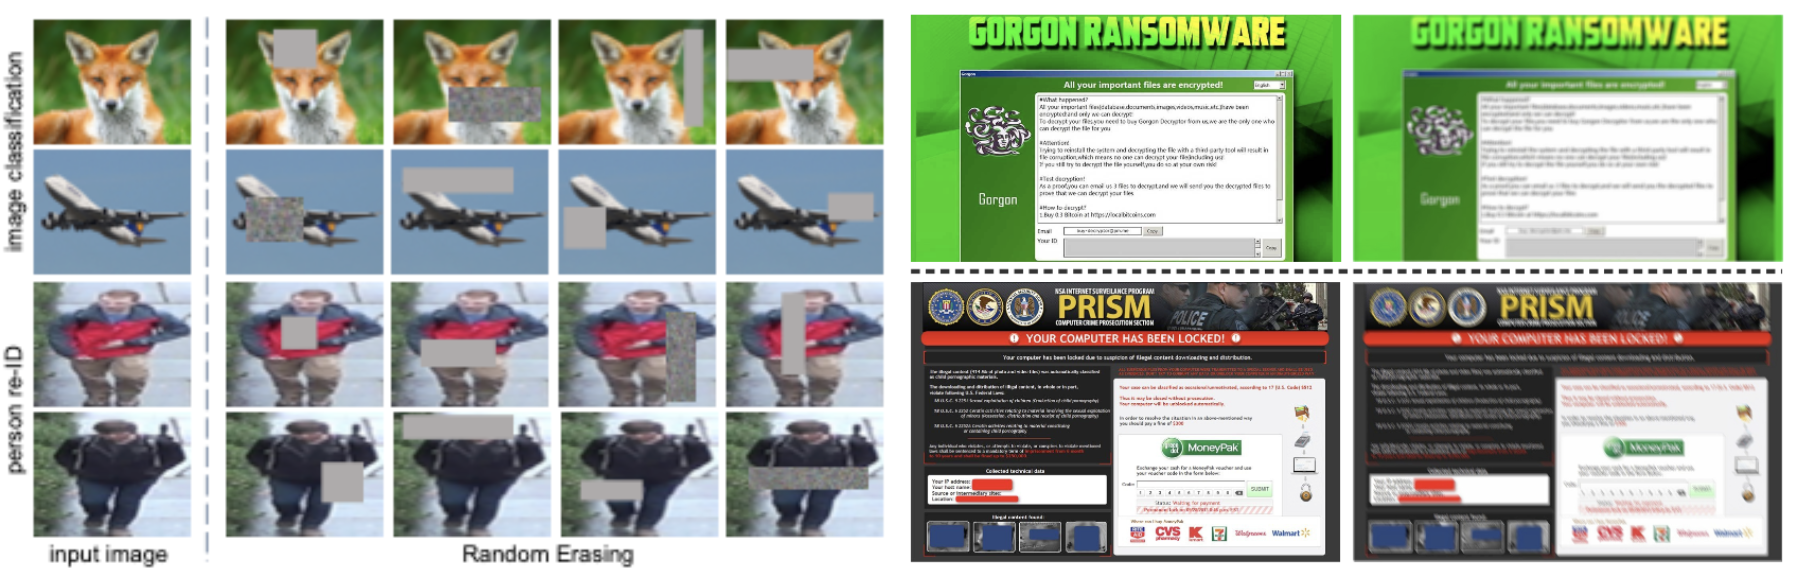
\includegraphics[scale=0.45]{Chapter4/figs/data-augs.png}
	\end{center}
	\caption[Examples of data augmentations found in the literature.]{Examples of data augmentations found in the literature. Left: randomly erasing parts of images, from Zhong \textit{et al}. \cite{zhong_random_2017}. Right: augmentations to simulate screenshot capture. Defocus blur (Top), motion blur (Bottom) from Atapour-Abarghouei \textit{et al}. \cite{atapour-abarghouei_kings_2019}.}
	\label{fig:data-aug-examples}
\end{figure}

As the Zanzibar data contains relatively few images, it is a prime candidate for data augmentation. This can be performed in one of two ways; in either an offline or an online manner. In offline data augmentation, the entire train split is augmented before the images are passed to the model, occurring as a pre-processing step. The major issue with offline augmentations however is that, because the data is perturbed and then passed to the model, offline augmentation produces a fixed number of augmented images. 

This can be solved with online augmentation. Occurring in real-time as the model trains, this allows for a potentially unlimited number of `new' images, as each input is randomly perturbed before being used for training. Once training on the batch has been completed, the augmented images are discarded and new perturbations performed. As such online augmentation is, if possible, greatly preferred and allows for a much higher chance of model generalisation. 

Whilst the Zanzibar dataset is small compared to many others used for deep learning, it is large enough to allow for online augmentation. In order to begin testing the effect of data augmentation on the Mask R-CNN training process, two different augmentation strategies were created which contained unique workflows. 

The first strategy, \textit{aug1}, selected between zero and three of the following perturbations: (1) \textit{horizontal flip}: flip the image horizontally with a probability of 0.5, (2) \textit{vertical flip}: flip the image vertically with a probability of 0.5, (3) \textit{rotation}: rotate the image either 90, 180, or 270 degrees each with equal probability of occurring, (4) \textit{scaling}: scale the image between 80\% and 120\% on both axis independent of each other, (5) \textit{brightness}: multiply all pixels in the image with a random value between 0.8 and 1.5, (6) \textit{Gaussian blur}: blur the image with a Gaussian kernel with radius randomly assigned between 0 and  5. 

The second strategy, \textit{aug2}, was more complex, performing the following perturbations in a sequentially random order on 67\% of the images: (1) \textit{horizontal flip}: flip the image horizontally with a probability of 0.5, (2) \textit{cropping}: crop each side of the image randomly between 0\% and 10\% of the total side length, (3) \textit{Gaussian blur}: blur the image with a Gaussian kernel with radius randomly assigned between 0 and 2.5, with a probability of blurring of 0.5, (4) \textit{contrast}: strengthen or weaken the contrast of the image by a random factor between 0.75 and 1.5, (5) \textit{additive Gaussian noise}: sample the noise per channel -- adding noise to the colour of the pixels, (6) \textit{brightness}: multiply all pixels in the image with a random value between 0.8 and 1.2, (7) \textit{scaling}: scale the image between 80\% and 120\% on both axes independent of each other, (8) \textit{rotation}: rotate the image randomly between -180 and 180 degrees. 

The use of two augmenters allowed for evaluation on whether a simple or more complex augmentation strategy would be appropriate for this use case. By using multiple augmenters we can treat them as a hyperparameter of model training, allowing the augmenter chosen to be added to the search space.

\section{Mask R-CNN Model Selection}\label{ch:cetDet,sec:ModelSelection}

When training a Mask R-CNN model there are a large range of hyperparameters, or user defined values, which must be set before training can occur. These hyperparameters each have influence on the final model's performance, and can be broken down into two subgroups; detection hyperparameters influence the output of the model, and training hyperparameters which influence the training of the model. Thankfully most deep learning frameworks provide default values for most, if not all hyperparameters. These default values are known to work well regardless of dataset or task, and so many have been used when training the Mask R-CNN. Some hyperparameters however can have a large effect on the final model and so an exploration of the optimal value for these has been undertaken with the goal of producing the optimal overall model for the task of cetacean detection, both on the Zanzibar dataset and on other similar datasets. 

\subsection{Detection Hyperparameters}\label{ch:cetDet,sec:ModelSelection,sub:DetectionHyperparameters}
 
 With regards to the detection hyperparameters, only the minimum confidence of the model was changed from the default of 0.7 to 0.9. This was changed as during initial trials it was found that models trained on the Zanzibar data would often produce a high number of false positives (for example detecting a wave as a fin) or create duplicate detections (one fin detected twice). By increasing the minimum confidence of the model to 0.9, the threshold at which the model returns a detection is increased to 90\% -- or in other words, for every detection the model must be 90\% sure that the detection is actually a cetacean before notifying the user. This has the effect of reducing the number of erroneous detections passed downstream, such as in Figure \ref{fig:min-conf} where increasing the minimum confidence from 0.7 (Left) to 0.9 (Right) has removed a low confidence, erroneous, detection. 
 
\begin{figure}[h]
	\begin{center}
		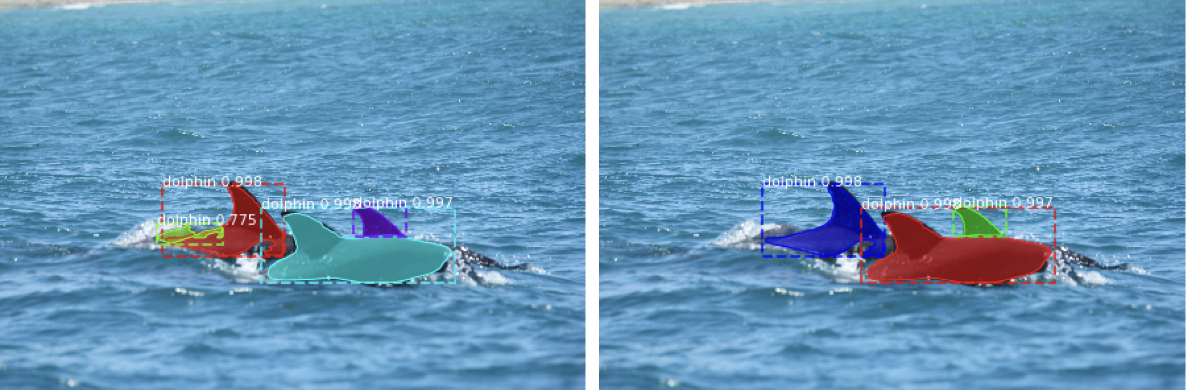
\includegraphics[scale=0.55]{Chapter4/figs/min-conf-eg.png}
	\end{center}
	\caption[An example image showing the effect of changing the Mask R-CNN's minimum detection confidence.]{An example image showing the effect of changing the Mask R-CNN's minimum detection confidence. Left: a threshold of 0.7. Right: a threshold of 0.9. The number of detections has reduced from four to three, with the erroneous left-most detection (highlighted green in the Left Figure) removed.}
	\label{fig:min-conf}
\end{figure}
 
 
\subsection{Training Hyperparameters}\label{ch:cetDet,sec:ModelSelection,sub:TrainingHyperparameters}

The vast majority of hyperparameters influence the training process. Selection of the optimal hyperparameters is however an extremely computationally and time expensive task, as the optimal values of the hyperparameters are not known before training begins. Indeed, even after training has finished and a model which produces satisfactory results has been found there is no guarantee that the hyperparameters of this model are the best, just that they are the best found so far. 

As such, in order to determine the best hyperparameters for a given model and task, the search space of all possible hyperparameters must be searched. This is infeasible due to time and resource constraints however, therefore a technique known as grid searching was performed. During a grid search, each hyperparameter is defined as a range of possible values. A model is then trained using the data and each combination of defined hyperparameter values. Once each model has trained, they are then evaluated using the test data to determine the best hyperparameters.

\subsubsection{Learning Rate Scheduling and Optimisers}\label{ch:cetDet,sec:ModelSelection,sub:TrainingHyperparameters,subsub:learningRateOptimisers}
One of the most important hyperparameters to tune is the learning rate, which dictates how much the weights of the model should change in response to the estimated error calculated during backpropagation. If the learning rate is too large this will lead to an unstable training process whereby gradient descent can never reach the minimum value but rather bounce either side of it. If the learning rate is set too small the training process will take an extremely long time to converge. 

In order to help the model reach its optimal minima in a reasonable time, the learning rate can be adjusted using a scheduler. These allow for the learning rate to be modified when some criteria is met, such as after a set number of epochs, allowing for larger weight changes initially for fast training before reducing the descent steps as time goes on, decreasing the chance of gradient descent jumping over the minima.

As well as learning rate schedulers, adaptive rate optimisers can also be used. These optimisers provide an alternative to SGD (an overview of which can be found in Section \ref{ch:Background,sec:DLIntro,sub:stochasticgradientdescent}) and are capable of adapting to the dataset it is given and the current training process, changing the learning rate without a defined schedule. This often allows for a more optimised and efficient training process when compared to using SGD, as discussed in Section \ref{ch:Background,sec:DLIntro,sub:stochasticgradientdescent}. During hyperparameter tuning of the Mask R-CNN, two optimisers were chosen for evaluation. 

The first, SGD with restarts (SGDR) \cite{loshchilov_sgdr:_2016} allows for decreases in the learning rate through a process known as cosine annealing, whereby the decrease follows a cosine waveform. This results in a high starting learning rate allowing for a fast approach to a local minima before reducing the rate as the number of epochs increases to prevent a jump over the minima, similarly to how a scheduler works. However it may not be the case that this local minima is the global minima, the lowest possible point in the space. Due to cosine annealing it would not be possible to leave the local minima, the learning rate needs to be increased again to allow for this. As such the learning rate is \textit{restarted}, or increased back to its maximum, to allow for the training process to jump out of the local minima; if it is indeed the case that this local minima is also the global minima then the training process will return to the point it was at before the restart, however if the local minima was not the global minima, the restart will allow for the training process to leave the sub-optimal minima it previously found. 

The second learning rate optimisation explored during hyperparameter tuning is Adam, or adaptive moment estimation. This optimiser is extremely popular in the world of deep learning \cite{karpathy_peek_2017}, capable of achieving impressive results in relatively short training times. This is possible through the use of one learning rate for each model weight, in contrast to the singular learning rate for the whole model as seen in SGD or SGDR. Adam also utilises parts of other optimisers such as AdaGrad \cite{duchi_adaptive_2011} and RMSProp \cite{tieleman_lecture_2012} to allow the optimiser to work well with both sparse and noisy data. For a complete breakdown of the inner workings of Adam, see Kingma \textit{et al}. \cite{kingma_adam:_2014}. 

\subsubsection{Weight Decay}\label{ch:cetDet,sec:ModelSelection,sub:TrainingHyperparameters,subsub:WeightDecay}

The goal of neural network development is to utilise the training data in such a way that the resulting generated model performs well on unseen data. In order for this to be achieved the model must be generalisable, having learnt enough from the training data to perform well at the given task but not having learnt so well that it is unable to perform adequately on unseen data. If a model fails to generalise, it is said to have overfitted the data. For example, a model may be developed to detect cats in images, but is only presented with examples containing white cats. In this situation, the model may operate perfectly over the training and test data, however may fail when deployed to detect black cats. The model has learnt the training data too well and believes cats can only be white -- the model has overfitted. 

There are many different techniques to reduce overfitting in neural networks, one of the easiest is to simply collect more training data. As previously mentioned, due to how closely guarded cetacean photo-id catalogue data is and how expensive it is to collect, this was not possible. As such, the use of weight decay was explored during hyperparameter tuning. Weight decay is a regularisation technique which allows the model training to be penalised in proportion to the size of its weights. This incentivises the training process to keep the weights small, which has been shown to improve generalisation to unseen data \cite{krogh_simple_1991}. As the Zanzibar dataset is comparatively small compared to the usual size of datasets for this task, allowing the model to generalise well using small amounts of data is extremely important.

\subsubsection{Region Proposal Network Anchor Scales}\label{ch:cetDet,sec:ModelSelection,sub:TrainingHyperparameters,subsub:RPNAnchorScales}

As discussed in Section \ref{ch:Background,sec:objectDetection,sub:RPN}, Region Proposal Networks (RPNs) can be utilised in object detection due to their ability to determine potential regions of interest (RoIs) in the image, known as anchors. These anchors are then classified as either \texttt{background} or of a learnable class, such as \texttt{dolphin}. To allow the RPN to be object-size invariant, anchor scales are utilised. These scales, provided as a list of values which correspond to the square anchor size in pixels, determine what sizes the RoIs proposed by the RPN should be. For example, if an anchor scale of \texttt{[32]} is passed to the RPN, this would mean that all RoIs proposed by the RPN would be of size 32x32 pixels. The anchor scale provided to the RPN can be considered a hyperparameter as the best scales for the RPN to allow for the detection of objects regardless of their size must be determined. 

\subsection{Hyperparameter Tuning via Grid Search}\label{ch:cetDet,sec:ModelSelection,sub:HyperparameterTuning}

Although only a few hyperparameters have been chosen to tune, the size of the possible search space to evaluate is still extremely large. As mentioned previously, it is not feasible both from a time and resource perspective to evaluate the entire space and find the truly optimal value for each hyperparameter. Instead the search space is discretised using a grid search, for each hyperparameter a subset of possible values is selected. Each combination of hyperparameter values is then evaluated to determine which subset produces a satisfactory model. 

The list of models generated by the grid search, their hyperparameter combinations, and their mAP@IOU[0.5, 0.75, 0.85] scores can be seen in Table \ref{tab:MaskRCNNHyperparamTuningGridSearch}. This hyperparameter tuning run required a significant amount of time and resources, running over three cloud instance virtual machines (VMs)\nomenclature[z-VM]{VM}{Virtual Machine}, each with two Tesla K80 GPUs, taking approximately one week to produce a total of 50 models. Model runs were split between the VMs based on augmentation strategy with one VM running only \textit{aug1}, the other \textit{aug2}, and the final with no augmentation strategy. It should be noted here that this computational and time expense would most likely be reduced should the images used to train the Mask R-CNN not be so large, although the reasons for this decision are discussed in Section \ref{ch:cetDet,sec:requirements,sub:technical}.

\begin{table}[!ht]
	\tiny
	\begin{adjustbox}{width=\columnwidth, center}
		\begin{tabular}{ccccccccc}
			\hline
			\multirow{2}{*}{\textbf{Model Name}} & \multirow{2}{*}{\textbf{\textbf{\begin{tabular}[c]{@{}c@{}}Weight\\Decay\end{tabular}}}} & \multirow{2}{*}{\textbf{\textbf{\begin{tabular}[c]{@{}c@{}}RPN\\Anchor Scales\end{tabular}}}} & \multirow{2}{*}{\textbf{Optimiser}} & \multirow{2}{*}{\textbf{\begin{tabular}[c]{@{}c@{}}Augmentation\\Strategy\end{tabular}}} & \multirow{2}{*}{\textbf{\begin{tabular}[c]{@{}c@{}}Pre-trained on\\ MSCOCO?\end{tabular}}} & \multicolumn{3}{c}{\textbf{mAP@IOU[$x$]}}        \\ \cline{7-9} 
			&                                        &                                             &                                     &                                                                                           &                                                                                            & \textbf{0.50}   & \textbf{0.75}  & \textbf{0.85}  \\ \hline
			20190829T1458                        & $1\times10^{-2}$                                   & (16, 32, 64, 128, 256)                      & Adam                                & aug1                                                                                      & \cmark                                                                                     & 0.774          & 0.555          & 0.265          \\
			20190829T2020                        & $1\times10^{-2}$                                   & (16, 32, 64, 128, 256)                      & Adam                                & aug2                                                                                      & \cmark                                                                                     & 0.739          & 0.513          & 0.180          \\
			20190830T0145                        & $1\times10^{-2}$                                   & (16, 32, 64, 128, 256)                      & Adam                                & None                                                                                      & \cmark                                                                                     & 0.843          & 0.586          & 0.245          \\
			20190830T0714                        & $1\times10^{-2}$                                   & (16, 32, 64, 128, 256)                      & Adam                                & aug1                                                                                      & \xmark                                                                                     & 0.793          & 0.492          & 0.174          \\
			20190830T1443                        & $1\times10^{-2}$                                   & (16, 32, 64, 128, 256)                      & Adam                                & aug2                                                                                      & \xmark                                                                                     & 0.732          & 0.531          & 0.199          \\
			20190830T2019                        & $1\times10^{-2}$                                   & (16, 32, 64, 128, 256)                      & Adam                                & None                                                                                      & \xmark                                                                                     & 0.858          & 0.609          & 0.278          \\
			\textbf{20190902T0946}               & $\mathbf{1\times10^{-2}}$                         & \textbf{(16, 32, 64, 128, 256)}             & \textbf{SGDR}                       & \textbf{aug1}                                                                             & \textbf{\cmark}                                                                            & \textbf{0.914} & \textbf{0.793} & \textbf{0.497} \\
			20190904T2004                        & $1\times10^{-2}$                                   & (16, 32, 64, 128, 256)                      & SGDR                                & None                                                                                      & \cmark                                                                                     & 0.896          & 0.665          & 0.235          \\
			20190905T1813                        & $1\times10^{-3}$                                  & (32, 64, 128, 256, 512)                     & SGDR                                & aug1                                                                                      & \cmark                                                                                     & 0.937          & 0.775          & 0.452          \\
			20190905T1826                        & $1\times10^{-2}$                                   & (16, 32, 64, 128, 256)                      & SGDR                                & aug2                                                                                      & \cmark                                                                                     & 0.915          & 0.762          & 0.418          \\
			20190905T2202                        & $1\times10^{-3}$                                  & (32, 64, 128, 256, 512)                     & Adam                                & None                                                                                      & \cmark                                                                                     & 0.817          & 0.594          & 0.281          \\
			20190905T2336                        & $1\times10^{-3}$                                  & (32, 64, 128, 256, 512)                     & Adam                                & aug1                                                                                      & \cmark                                                                                     & 0.822          & 0.640          & 0.265          \\
			20190906T0332                        & $1\times10^{-3}$                                  & (32, 64, 128, 256, 512)                     & SGDR                                & None                                                                                      & \cmark                                                                                     & 0.902          & 0.738          & 0.417          \\
			20190906T0851                        & $1\times10^{-2}$                                   & (32, 64, 128, 256, 512)                     & Adam                                & None                                                                                      & \cmark                                                                                     & 0.856          & 0.640          & 0.277          \\
			20190907T0932                        & $1\times10^{-3}$                                  & (16, 32, 64, 128, 256)                      & Adam                                & aug1                                                                                      & \cmark                                                                                     & 0.834          & 0.567          & 0.239          \\
			20190907T0933                        & $1\times10^{-4}$                                 & (32, 64, 128, 256, 512)                     & Adam                                & aug2                                                                                      & \xmark                                                                                     & 0.844          & 0.592          & 0.243          \\
			20190907T0934                        & $1\times10^{-2}$                                   & (32, 64, 128, 256, 512)                     & SGDR                                & None                                                                                      & \xmark                                                                                     & 0.921          & 0.796          & 0.457          \\
			20190907T1451                        & $1\times10^{-3}$                                  & (16, 32, 64, 128, 256)                      & Adam                                & None                                                                                      & \cmark                                                                                     & 0.804          & 0.560          & 0.197          \\
			20190907T1500                        & $1\times10^{-4}$                                 & (32, 64, 128, 256, 512)                     & Adam                                & aug1                                                                                      & \xmark                                                                                     & 0.837          & 0.649          & 0.289          \\
			20190907T1545                        & $1\times10^{-2}$                                   & (32, 64, 128, 256, 512)                     & Adam                                & aug2                                                                                      & \xmark                                                                                     & 0.850          & 0.612          & 0.229          \\
			20190907T2026                        & $1\times10^{-4}$                                 & (32, 64, 128, 256, 512)                     & SGDR                                & None                                                                                      & \cmark                                                                                     & 0.919          & 0.782          & 0.412          \\
			20190907T2126                        & $1\times10^{-3}$                                  & (16, 32, 64, 128, 256)                      & Adam                                & aug1                                                                                      & \xmark                                                                                     & 0.827          & 0.544          & 0.257          \\
			20190907T2215                        & $1\times10^{-3}$                                  & (16, 32, 64, 128, 256)                      & SGDR                                & aug2                                                                                      & \cmark                                                                                     & 0.928          & 0.789          & 0.452          \\
			20190908T0202                        & $1\times10^{-4}$                                 & (16, 32, 64, 128, 256)                      & Adam                                & None                                                                                      & \cmark                                                                                     & 0.848          & 0.619          & 0.281          \\
			20190908T0352                        & $1\times10^{-2}$                                   & (32, 64, 128, 256)                          & Adam                                & aug2                                                                                      & \cmark                                                                                     & 0.836          & 0.566          & 0.259          \\
			20190908T0417                        & $1\times10^{-4}$                                 & (32, 64, 128, 256, 512)                     & Adam                                & aug1                                                                                      & \cmark                                                                                     & 0.827          & 0.619          & 0.287          \\
			20190908T0957                        & $1\times10^{-4}$                                 & (32, 64, 128, 256, 512)                     & Adam                                & None                                                                                      & \xmark                                                                                     & 0.884          & 0.681          & 0.324          \\
			20190908T1102                        & $1\times10^{-4}$                                 & (32, 64, 128, 256, 512)                     & Adam                                & aug2                                                                                      & \xmark                                                                                     & 0.790          & 0.581          & 0.256          \\
			20190908T1204                        & $1\times10^{-3}$                                  & (16, 32, 64, 128, 256)                      & SGDR                                & aug1                                                                                      & \cmark                                                                                     & 0.901          & 0.733          & 0.453          \\
			20190908T1939                        & $1\times10^{-3}$                                  & (16, 32, 64, 128, 256)                      & Adam                                & aug2                                                                                      & \xmark                                                                                     & 0.811          & 0.579          & 0.203          \\
			20190908T2043                        & $1\times10^{-4}$                                 & (32, 64, 128, 256, 512)                     & SGDR                                & aug1                                                                                      & \cmark                                                                                     & 0.929          & 0.804          & 0.482          \\
			20190908T2139                        & $1\times10^{-4}$                                 & (16, 32, 64, 128, 256)                      & Adam                                & None                                                                                      & \xmark                                                                                     & 0.910          & 0.686          & 0.349          \\
			20190909T0723                        & $1\times10^{-4}$                                 & (16, 32, 64, 128, 256)                      & Adam                                & aug1                                                                                      & \xmark                                                                                     & 0.798          & 0.644          & 0.298          \\
			20190911T1922                        & $1\times10^{-2}$                                   & (16, 32, 64, 128, 256)                      & Adam                                & aug2                                                                                      & \xmark                                                                                     & 0.765          & 0.508          & 0.174          \\
			20190912T0045                        & $1\times10^{-4}$                                 & (16, 32, 64, 128, 256)                      & Adam                                & aug2                                                                                      & \xmark                                                                                     & 0.780          & 0.539          & 0.214          \\
			20190912T0608                        & $1\times10^{-4}$                                 & (16, 32, 64, 128, 256)                      & SGDR                                & aug1                                                                                      & \cmark                                                                                     & 0.910          & 0.771          & 0.463          \\
			20191101T1633                        & $1\times10^{-4}$                                 & (32, 64, 128, 256, 512)                     & SGDR                                & aug2                                                                                      & \cmark                                                                                     & 0.909          & 0.780          & 0.419          \\
			20191101T2104                        & $1\times10^{-3}$                                  & (8, 16, 32, 64, 128)                        & SGDR                                & aug2                                                                                      & \cmark                                                                                     & 0.901          & 0.750          & 0.340          \\
			20191102T0140                        & $1\times10^{-2}$                                   & (32, 64, 128, 256, 512)                     & SGDR                                & aug1                                                                                      & \cmark                                                                                     & 0.916          & 0.813          & 0.442          \\
			20191102T0615                        & $1\times10^{-2}$                                   & (8, 16, 32, 64, 128)                        & SGDR                                & aug2                                                                                      & \cmark                                                                                     & 0.902          & 0.745          & 0.410          \\
			20191102T1051                        & $1\times10^{-4}$                                 & (16, 32, 64, 128, 256)                      & SGDR                                & None                                                                                      & \xmark                                                                                     & 0.914          & 0.812          & 0.461          \\
			20191102T1528                        & $1\times10^{-3}$                                  & (32, 64, 128, 256, 512)                     & SGDR                                & aug2                                                                                      & \cmark                                                                                     & 0.919          & 0.778          & 0.425          \\
			20191102T2006                        & $1\times10^{-4}$                                 & (8, 16, 32, 64, 128)                        & SGDR                                & aug2                                                                                      & \cmark                                                                                     & 0.919          & 0.747          & 0.391          \\
			20191103T0044                        & $1\times10^{-4}$                                 & (8, 16, 32, 64, 128)                        & SGDR                                & aug1                                                                                      & \cmark                                                                                     & 0.901          & 0.736          & 0.348          \\
			20191103T0520                        & $1\times10^{-3}$                                  & (8, 16, 32, 64, 128)                        & SGDR                                & None                                                                                      & \cmark                                                                                     & 0.913          & 0.778          & 0.443          \\
			20191103T0959                        & $1\times10^{-2}$                                   & (32, 64, 128, 256, 512)                     & SGDR                                & aug2                                                                                      & \cmark                                                                                     & 0.929          & 0.766          & 0.437          \\
			20191103T1441                        & $1\times10^{-4}$                                 & (8, 16, 32, 64, 128)                        & SGDR                                & None                                                                                      & \cmark                                                                                     & 0.882          & 0.739          & 0.401          \\
			20191103T1921                        & $1\times10^{-4}$                                 & (16, 32, 64, 128, 256)                      & SGDR                                & aug2                                                                                      & \cmark                                                                                     & 0.926          & 0.768          & 0.360          \\
			20191104T0011                        & $1\times10^{-3}$                                  & (8, 16, 32, 64, 128)                        & SGDR                                & aug1                                                                                      & \cmark                                                                                     & 0.912          & 0.788          & 0.391          \\
			20191104T0450                        & $1\times10^{-2}$                                   & (8, 16, 32, 64, 128)                        & SGDR                                & aug1                                                                                      & \cmark                                                                                     & 0.915          & 0.782          & 0.394          \\ \hline
		\end{tabular}
	\end{adjustbox}
	\caption[Hyperparameter values and mAP@IOU{[}0.5, 0.75, 0.85{]} scores used for each Mask R-CNN grid search model trained on the Zanzibar data.]{Hyperparameter values and mAP@IOU{[}0.5, 0.75, 0.85{]} scores used for each Mask R-CNN grid search model trained on the Zanzibar data. All models were trained for 50 epochs with an initial learning rate of $1\times10^{-3}$. The model chosen for use is highlighted in bold. The mAP@IOU{[}0.5:0.95{]} scores for all models can be seen in Appendix \ref{app:mAPScoresGridSearch}.}\label{tab:MaskRCNNHyperparamTuningGridSearch}
\end{table}

\subsection{Model Selection Based on Grid Search}\label{ch:cetDet,sec:ModelSelection,sub:ModelSelectionBasedOnGridSearch}

Once a grid search has been performed, the results can then be evaluated to determine if a suitable model had been found using the test set. All models trained were evaluated using MSCOCO's Mean Average Precision metric\footnote{COCO mAP Definition: \href{https://cocodataset.org/\#detection-eval}{cocodataset.org/\#detection-eval}}, a commonly used metric for segmentation tasks. This metric, written as mAP@IOU[0.5:0.95], calculates precision-recall graphs for each dataset class at incremental IOU levels, from 0.5 to 0.95 in 0.05 steps. Once each class' precision-recall graph for a given IOU threshold has been calculated, the mean of these values is derived giving an overall mean average precision score for all classes at a given IOU threshold; these thresholds are explained in more detail in Section \ref{ch:Background,sec:semanticSegmentation}. Appendix \ref{app:mAPScoresGridSearch} provides the full mAP@IOU[0.5:0.95] scores for all models trained in the grid search.

By evaluating over multiple thresholds the models can then be compared and their performance more easily understood and ranked, as well as allow for the determination of an acceptable loss in IOU overlap. For example if all models were evaluated using mAP@IOU[0.5] only, it may be the case that all models achieve a similar high score, making it difficult to determine which model will be best for the task. However if too high a threshold is used, for example mAPIOU[0.95], it is unlikely that any model will achieve a high score as this constant near pixel perfect detection. 

At mAP@IOU[0.5] there is a large gap in model performance with model 20190830T1443 having the lowest mAP@IOU[0.5] of 0.73 and model 20190905T1813 having the highest at 0.94. This shows that the combination of hyperparameter values provided to the model before training have a significant effect on the model's overall performance, although even the lowest score here is still high. 

At mAP@IOU[0.75], whereby detections would overlap with 75\% of pixels in the ground truth mask, the minimum model performance has dropped significantly with model 20190830T071 achieving a score of 0.49. The highest score at this threshold is model 20191102T0140 with a score of 0.81; this model achieved an mAP@IOU[0.5] score of 0.92, only two percentage points behind the best model at that threshold. This again shows the need for hyperparameter tuning when selecting models, as they are shown here to have a significant effect on how well the models perform at higher thresholds.

This effect is even greater when comparing map@IOU[0.85] scores, with the worst performing model, 20190830T0714,  achieving a score of just 0.17 whilst the best model, 20190902T0946, achieves a score of 0.50, a difference of 33\%. Model performance drops significantly at the highest threshold with four models achieving an mAP@IOU[0.95] score of 0.016, with most models achieving a score of 0.0. This is to be expected however as it would be highly unlikely that any model, regardless of hyperparameters, would be able to perform near perfect pixel level detections on the test set data. 

To determine the most appropriate model trained, filtering based on the highest mAP@IOU[0.5, 0.75, 0.85] scores was performed. The thresholds 0.5 and 0.75 were chosen to remain consistent with other segmentation literature \cite{bolya_yolact_2019, wang_solov2_2020, tian_fcos_2019}, with the 0.85 threshold chosen as some models trained still achieve impressive results here, allowing for more in-depth model filtering. Further, the pixel-wise detections of cetaceans is required to filter as much background noise as possible and so finding high performing models at top thresholds is important.

When filtering, the top five performing models at each threshold were extracted. If a model achieved top five ranking at multiple thresholds it was only included once, resulting in a list of the ten best performing models. The hyperparameters and mAP@IOU[0.5, 0.75, 0.85] scores for these best performing models can be seen in Table \ref{tab:best-mask-rcnn-models}.

\begin{table}[!ht]
	\tiny
	\begin{adjustbox}{width=\columnwidth, center}
		\begin{tabular}{ccccccccc}
			\hline
			\multirow{2}{*}{\textbf{Model Name}} & \multirow{2}{*}{\textbf{\textbf{\begin{tabular}[c]{@{}c@{}}Weight\\Decay\end{tabular}}}} & \multirow{2}{*}{\textbf{\textbf{\begin{tabular}[c]{@{}c@{}}RPN\\Anchor Scales\end{tabular}}}} & \multirow{2}{*}{\textbf{Optimiser}} & \multirow{2}{*}{\textbf{\begin{tabular}[c]{@{}c@{}}Augmentation\\Strategy\end{tabular}}} & \multirow{2}{*}{\textbf{\begin{tabular}[c]{@{}c@{}}Pre-trained on\\ MSCOCO?\end{tabular}}} & \multicolumn{3}{c}{\textbf{mAP@IOU[$x$]}}        \\ \cline{7-9} 
			&                                        &                                             &                                     &                                                                                           &                                                                                            & \textbf{0.50}   & \textbf{0.75}  & \textbf{0.85}  \\ \hline
			\textbf{20190902T0946} &         $\mathbf{1\times10^{-2}}$ &  \textbf{ (16, 32, 64, 128, 256)} &      \textbf{SGDR} &                  \textbf{aug1} &                  \textbf{\cmark} & 0.914 & 0.793 & 0.497\\
			20190905T1813 &        $1\times10^{-3}$ &  (32, 64, 128, 256, 512) &      SGDR &                  aug1 &                  \cmark & 0.937 & 0.775 & 0.452\\
			20190907T0934 &         $1\times10^{-2}$ &  (32, 64, 128, 256, 512) &      SGDR &                  None &                  \cmark & 0.921 & 0.796 & 0.452\\
			20190907T2215 &        $1\times10^{-3}$ &   (16, 32, 64, 128, 256) &      SGDR &                  aug2 &                  \cmark & 0.928 & 0.796 & 0.457\\
			20190908T2043 &       $1\times10^{-4}$ &  (32, 64, 128, 256, 512) &      SGDR &                  aug1 &                  \cmark & 0.929 & 0.804 & 0.482\\
			20190912T0608 &       $1\times10^{-4}$ &   (16, 32, 64, 128, 256) &      SGDR &                  aug1 &                  \cmark & 0.910 & 0.771 & 0.463 \\
			20191102T0140 &         $1\times10^{-2}$ &  (32, 64, 128, 256, 512) &      SGDR &                  aug1 &                  \cmark & 0.916 & 0.813 & 0.442\\
			20191102T1051 &       $1\times10^{-4}$ &   (16, 32, 64, 128, 256) &      SGDR &                  None &                  \cmark & 0.914 & 0.812 & 0.461\\
			20191103T0959 &         $1\times10^{-2}$ &  (32, 64, 128, 256, 512) &      SGDR &                  aug2 &                  \cmark & 0.929 & 0.766 & 0.437\\
			20191103T1921 &       $1\times10^{-4}$ &   (16, 32, 64, 128, 256) &      SGDR &                  aug2 &                  \cmark & 0.926 & 0.768 & 0.360\\
			\bottomrule
		\end{tabular}
	\end{adjustbox}
	\caption[Hyperparameters of the best performing Mask R-CNN models on the Zanzibar dataset.]{Hyperparameters of the best performing Mask R-CNN models on the Zanzibar dataset. Subset of Table \ref{tab:MaskRCNNHyperparamTuningGridSearch}. All models were trained for 50 epochs with an initial learning rate of $1\times10^{-3}$. The model chosen for use is highlighted in bold. The mAP@IOU{[}0.5:0.95{]} scores for all models can be seen in Appendix \ref{app:mAPScoresGridSearch}.}
	\label{tab:best-mask-rcnn-models}
\end{table}

When deciding on which model hyperparameters are best for the task of cetacean segmentation, it is important to find a model with a high mAP@IOU[0.85] score. As the model will be used to perform segmentation before fine-grained classification, it is important the model is capable of removing as much background from the input image as possible. Any background included in the segmentation may adversely effect the photo-id process. Using this as criteria, model 20190902T0946 was selected as the best performing model. The model achieves an mAP@IOU[0.85] score of 0.5, an excellent result given the difficulty of the segmentation task. The model also performs well at the other evaluation thresholds, achieving mAP@IOU[0.5, 0.75] scores of 0.91 and 0.79 respectively. These scores verify that the model is capable of segmenting cetaceans from background with as little noise being included in the segmentation mask as possible.

An interesting point to note here is that 20190902T0946 did not achieve the highest mAP@IOU[0.5, 0.75] scores. As previously mentioned, these thresholds are often the ones included in segmentation literature to evaluate model performance. If just these thresholds were used for model selection, 20190902T0946 would not have been chosen. This highlights the need to select models based on metrics which make sense for the task at hand. As the model is required to remove as much background noise as possible, using a high threshold for evaluation makes sense. Thresholds higher than 0.85 were not utilised due to the low performance of all models at this threshold, although 20190902T0946 also achieves one of the best mAP@IOU[0.9] scores of 0.150. Only one model, 20191102T0615 achieves a better score at this threshold, 0.158, however this model achieves lower performance at the chosen evaluation thresholds of 0.5, 0.75, and 0.85.

\subsection{An Evaluation of Optimal Model Hyperparameters}\label{ch:cetDet,sec:ModelSelection,sub:OptimalHyperparameters}

As discussed in Section \ref{ch:cetDet,sec:ModelSelection,sub:ModelSelectionBasedOnGridSearch} a filtering of the trained Mask R-CNN models was performed to determine the best model hyperparameters for the task of cetacean instance segmentation, with model 20190902T0946 ultimately being selected for future use. Model hyperparameters and mAP@IOU[0.5, 0.75, 0.85] scores can be seen in Table \ref{tab:best-mask-rcnn-models}.

The hyperparameters of the best performing models provide an interesting insight into the training process. All ten of the models were trained using SGDR. This is interesting, as the current trend in deep learning network training is to utilise Adam \cite{karpathy_peek_2017}. Furthermore each model trained utilised transfer learning, with each model's parameters being initialised from a trained MSCOCO model provided by the model zoo. This highlights the need to utilise pre-trained models, especially in cases where relativity small amounts of data are available to train a model from scratch. 

Half of the best models utilise the \textit{aug1} data augmentation strategy, defined in Section \ref{ch:cetDet,sec:initialTesting,sub:dataaugmentation}. The smallest RPN Anchor Scale, (8, 16, 32, 64, 128), has not been utilised by any of the best models, and the value of the weight decay hyperparameter is split between the three possible values. These splits highlight the need for a robust and in-depth hyperparameter search, as with the majority of hyperparameters searched no clear trend can be identified.

\subsection{Limitations of the Model}\label{ch:cetDet,sec:ModelSelection,sub:LimitationsOfBest}

As with any network trained on real world data, the best performing model, 20190902T0946, is not perfect. As highlighted by the mAP scores in Table \ref{tab:MaskRCNNHyperparamTuningGridSearch}, the model still fails to correctly detect in some instances. This section examines under what conditions 20190902T0946 fails for the purposes of model transparency. 

Figure \ref{fig:model-fail-bad-detection-and-split-individual} provides a good example of environmental conditions which can cause the model to fail to correctly detect an individual. Due to wave movement covering a part of the animal's body, the model has split this individual into two separate detections.

\begin{figure}[h]
	\begin{center}
		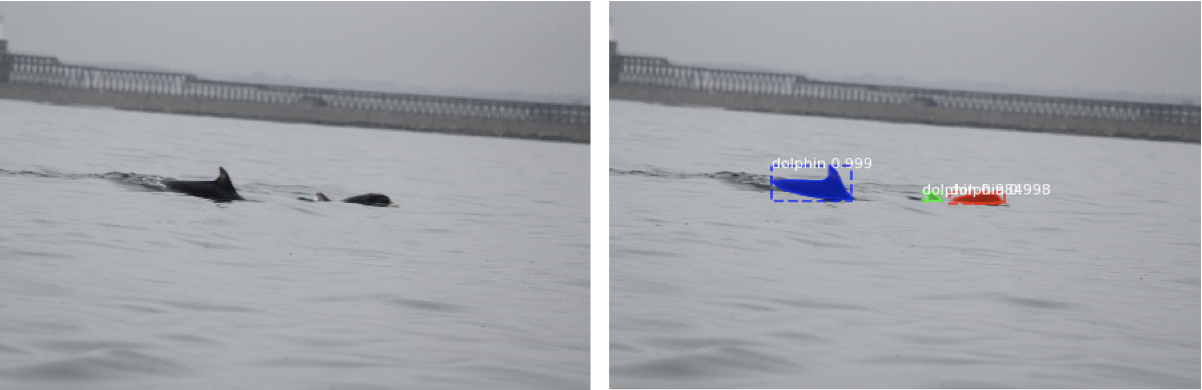
\includegraphics[scale=0.6]{Chapter4/figs/model-fail-split-individual.png}
	\end{center}
	\caption[Left: the input image passed to the cetacean detector. Right: the detection masks produced by the model overlaid onto the image.]{Left: the input image passed to the cetacean detector. Right: the detection masks produced by the model overlaid onto the image. Note how the cetacean on the right has been split over two masks due to occlusion from a small wave.}
	\label{fig:model-fail-bad-detection-and-split-individual}
\end{figure}
 
The model also struggles in cases where the image contains an animal under the waterline but, due to the clarity of the water, that animal is partly visible in the image. In this case the model often detects the individual under the waterline. Due to these individuals not being useful for identification purposes however, they were not labelled in the dataset and thus are deemed to be misclassifications when evaluating the model. Figure \ref{fig:model-fail-underwater} shows an example of this issue occurring.

\begin{figure}[h]
	\begin{center}
		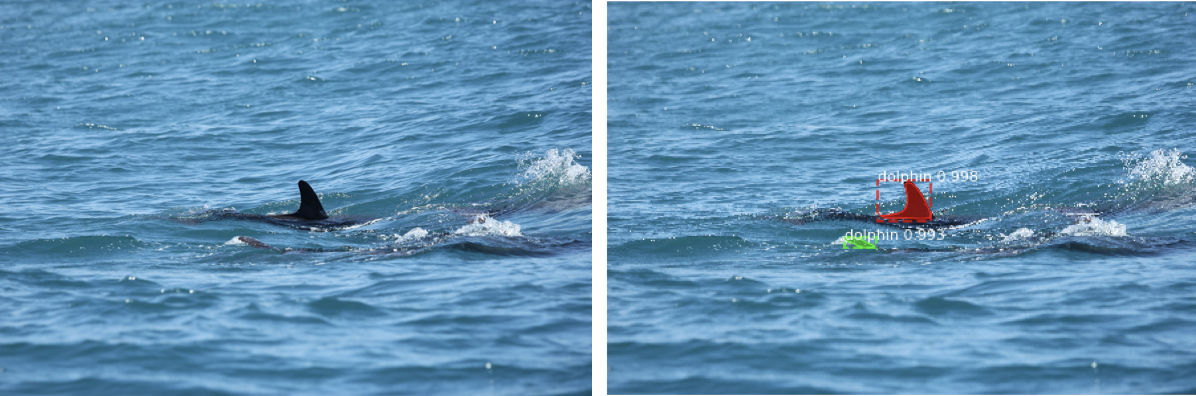
\includegraphics[scale=0.6]{Chapter4/figs/model-fail-underwater.png}
	\end{center}
	\caption[Left: the image passed to the cetacean detector. Right: the detection masks produced by the model overlaid onto the image.]{Left: the image passed to the cetacean detector. Right: the detection masks produced by the model overlaid onto the image. Note how the green detection is of an individual under the waterline and only partly visible, and thus useless for identification purposes. }
	\label{fig:model-fail-underwater}
\end{figure}

The Zanzibar dataset contains a large number of images which contain other vessels as well as dolphins. This is due to the large marine eco-tourism industry within Zanzibar \cite{sharpe_indian_2019, berggren_sustainable_2007}. Whilst this issue may not be present in other survey areas where this model may be deployed, it still denotes an example of the model failing. In this case often parts of the boat, or a combination of the boat and the humans on the boat, may cause the model to incorrectly identify a grouping of pixels as a dolphin. An example of this can be seen in Figure \ref{fig:model-fail-boat}.
 
\begin{figure}[h]
	\begin{center}
		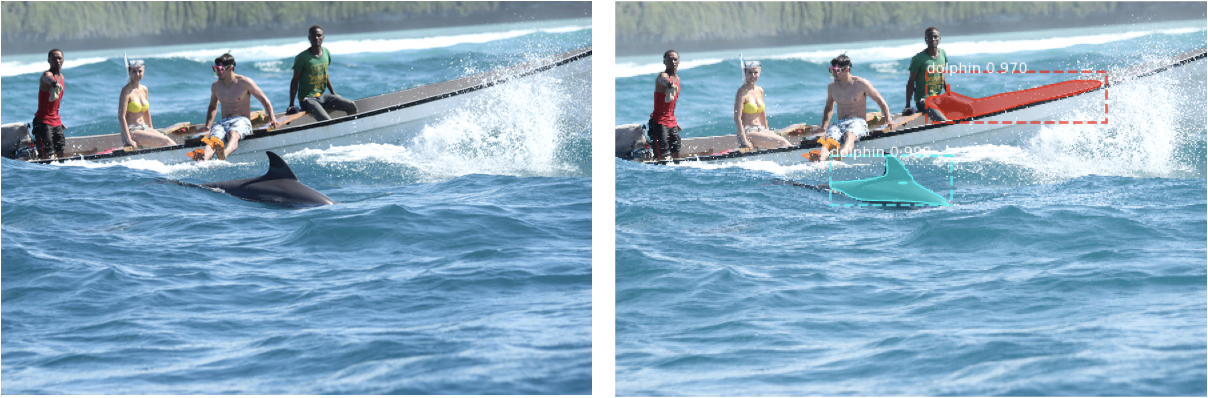
\includegraphics[scale=0.6]{Chapter4/figs/model-fail-boat.png}
	\end{center}
	\caption[Left: the image passed to the cetacean detector. Right: the detection masks produced by the model overlaid onto the image.]{Left: the image passed to the cetacean detector. Right: the detection masks produced by the model overlaid onto the image. Note how the red detection is a misclassification. The model believes a section of the boat's hull and the leg of the human to be a dolphin.}
	\label{fig:model-fail-boat}
\end{figure}

All of these mis-detections have an impact of the overall evaluation score of the model. These mis-detections will then be passed further down the system pipeline to be classified as individuals. To reduce the chances of this happening, a robust post-processing technique was developed, as discussed in Chapter \ref{ch:postProcessing}.

\section{Model Evaluation Using NDD20}\label{ch:cetDet,sec:EvalUsingNDD20}

To examine the dorsal fin detector's robustness to changes in geography, time, and species, evaluation of the model was then undertaken using the NDD20 dataset.

\subsection{Evaluating the Effect of Geography, Time, and Species Change}\label{ch:cetDet,sec:EvalUsingNDD20,subsec:geographyTimeSpeciesChange}

As discussed previously, a Mask R-CNN model capable of above water cetacean detection was trained on indo-pacific bottlenose dolphin data collected in Zanzibar, Tanzania. One important requirement of the detector created is that it must be robust enough to output detection masks with high mean average precision (mAP) when operating on data from a different geographic or temporal area without re-training. The creation of NDD20 provides a valuable opportunity to test this requirement. Not only was the data collected in a different location and time, but both species of data subject (bottlenose and white-beaked dolphin) are not present in the Zanzibar dataset.  

To test this requirement the best performing model found on the Zanzibar data in Section \ref{ch:cetDet,sec:ModelSelection,sub:ModelSelectionBasedOnGridSearch}, 20190902T0946, was utilised to generate instance segmentation mask predictions for the above water set of NDD20. These model outputs were then evaluated against the labelled ground truth data to produce an mAP score over multiple IOU thresholds.

Model 20190902T0946 still achieves a high mAP at multiple IOU thresholds without the need for re-training or fine-tuning on NDD20, as seen in Table \ref{tab:maskrcnn_results}. Utilising the same evaluation thresholds as during model selection in Section \ref{ch:cetDet,sec:ModelSelection,sub:ModelSelectionBasedOnGridSearch}, the model achieves mAP@IOU[0.5, 0.75] = [0.96, 0.83] on NDD20. This is in comparison to mAP@IOU[0.5, 0.75] = [0.91, 0.79] on the Zanzibar data.

\begin{table}
	\begin{adjustbox}{width=\linewidth, center}
		\begin{tabular}{ccccccccccc}
			\hline
			\multirow{2}{*}{\textbf{Dataset}} & \multicolumn{10}{c}{\textbf{mAP@IOU[$x$]}}                                                                                                                  \\
			& \textbf{0.50} & \textbf{0.55} & \textbf{0.60} & \textbf{0.65} & \textbf{0.70} & \textbf{0.75} & \textbf{0.80} & \textbf{0.85} & \textbf{0.90} & \textbf{0.95} \\ \hline
			\textbf{\begin{tabular}[t]{@{}c@{}}Zanzibar\\ (Test Set)\end{tabular}}                 & 0.91          & 0.91          & 0.89          & 0.86          & 0.85          & 0.79          & 0.69          & 0.50          & 0.15          & 0.00           \\
			\textbf{\begin{tabular}[t]{@{}c@{}}NDD20\\ (Above Water)\end{tabular}}                      & 0.96          & 0.95          & 0.93          & 0.91          & 0.88          & 0.83          & 0.71          & 0.51          & 0.16          & 0.00          \\ \hline
		\end{tabular}
	\end{adjustbox}
	\caption[mAP@IOU{[}0.5:0.95{]} scores for model 20190902T0946, the best performing Mask R-CNN dorsal fin detector.]{mAP@IOU{[}0.5:0.95{]} scores for model 20190902T0946, the best performing Mask R-CNN dorsal fin detector. The model has been trained using the Zanzibar training set, and evaluated using both the Zanzibar test set and the full NDD20 above water set. Hyperparameters for this model can be seen in Table \ref{tab:MaskRCNNHyperparamTuningGridSearch}.}
	\label{tab:maskrcnn_results}
\end{table}

Interestingly, the model achieves a higher mAP at these IOU thresholds on NDD20. This is hypothesised to be due to the lack of other large objects in NDD20 in comparison to the Zanzibar data. For example, some images in the Zanzibar dataset contain other vessels as well as humans as a result of the data being captured in an area with high levels of eco-tourism \cite{christiansen_effects_2010}. This is not the case for data contained within NDD20. Whilst eco-tourism is present in and around the Coquet to St. Mary's MCZ, the levels are significantly lower than in Zanzibar. The evaluated model has been seen to struggle when presented with images containing tourist activity, shown in Figure \ref{fig:model-fail-boat}. As NDD20 lacks this, the model's false positive rate may be reduced. Regardless, this evaluation presents evidence that model 20190902T0946 is robust enough to deal with data from a different geographic area, time, and cetacean species without the need for re-training or fine-tuning. This suggests the model could be deployed to aid in the speed up of future photo-id fieldwork seasons undertaken by marine ecologists. 

\subsection{Below Water Detection Baseline}\label{ch:cetDet,sec:EvalUsingNDD20,subsec:belowWaterDetectionBasleine}

Though the below water set of NDD20 is not utilised within this thesis further, work was also undertaken to produce a baseline instance segmentation score for this data. Here, a second Mask R-CNN model was trained using the optimal hyperparameters located in Section \ref{ch:cetDet,sec:ModelSelection} on the below water data divided randomly into an 80:20 train-test split, with the \texttt{out of focus} flag ignored. Results for this model can be seen in Table \ref{tab:bw_results}, and indicate that a Mask R-CNN model is capable of accurate instance segmentation on this data -- in spite of the large variation in mask shape and a lack of clarity between the background and the dolphin due to water condition. 

\begin{table}[!h]
	\begin{adjustbox}{width=\linewidth, center}
		\begin{tabular}{ccccccccccc}
			\hline
			\multirow{2}{*}{\textbf{Dataset}} & \multicolumn{10}{c}{\textbf{mAP@IOU[$x$]}}                                                                                                                  \\
			& \textbf{0.50} & \textbf{0.55} & \textbf{0.60} & \textbf{0.65} & \textbf{0.70} & \textbf{0.75} & \textbf{0.80} & \textbf{0.85} & \textbf{0.90} & \textbf{0.95} \\ \hline
			\textbf{\begin{tabular}[t]{@{}c@{}}NDD20\\ (Below Water)\end{tabular}}                      & 0.986          & 0.982          & 0.979          & 0.974          & 0.964          & 0.938          & 0.871          & 0.654          & 0.202          & 0.00          \\ \hline
		\end{tabular}
	\end{adjustbox}
	\caption{mAP@IOU{[}0.5:0.95{]} scores for the best performing Mask R-CNN model trained using the below water set of NDD20.}
	\label{tab:bw_results}
\end{table}

\section{Summary}\label{ch:cetDet,sec:Summary}

This chapter discusses the thesis' need for a model capable of cetacean detection, both from a technical and environmental perspective. The key reasons behind the use of instance segmentation masks rather than the relatively less computational and time expensive bounding boxes is explained, with evidence showing how the difficulty of the task influenced this move. 

Once the system requirements and underlying model architecture have been identified, the chapter then examines the use of model hyperparameter optimisation to train a model capable of cetacean detection via instance segmentation masks contained in the Zanzibar dataset (outlined in Section \ref{ch:datasetCreation,sec:zanzibar}). Model pre-training is also explored, and highlights the benefits of this approach even when using a pretraining dataset whose domain and distribution are vastly different to the final model's goal. The chapter then examines the use of post-processing techniques to improve the output of the Mask R-CNN's detections for use in downstream tasks. 

It is of great importance that the trained Mask R-CNN model is capable of detecting cetaceans in photo-id data which has been gathered in different geospatial and temporal areas. It is also important that the detector is capable of similarly high levels of accuracy without re-training on data from that geographic area. As such, the detector's use on the NDD20 dataset, collected in a different geospatial and temporal area (outlined in Section \ref{ch:datasetCreation,sec:NDD}), is explored. The final result of this chapter is a Mask R-CNN model capable of high mAP even at large IoU thresholds. 

Before dorsal fin detections produced by the Mask R-CNN model developed in this chapter can be passed to a most likely catalogue matching system, some post-processing of the output must be performed. This will allow for the retention of any individually identifying markings potentially missed by the model's binary output mask, as well as allow for a reduction in the size of the input passed for catalogue matching, reducing downstream computational expense. This post-processing methodology is outlined in Chapter \ref{ch:postProcessing}.

%%%%%%%%%%%%%%%%%%%
